\documentclass{standalone}
\usepackage{pgfplots}
\pgfplotsset{width=10cm,compat=1.9}
%\usepgfplotslibrary{external}
%\tikzexternalize[prefix=tikz/]
\begin{document}


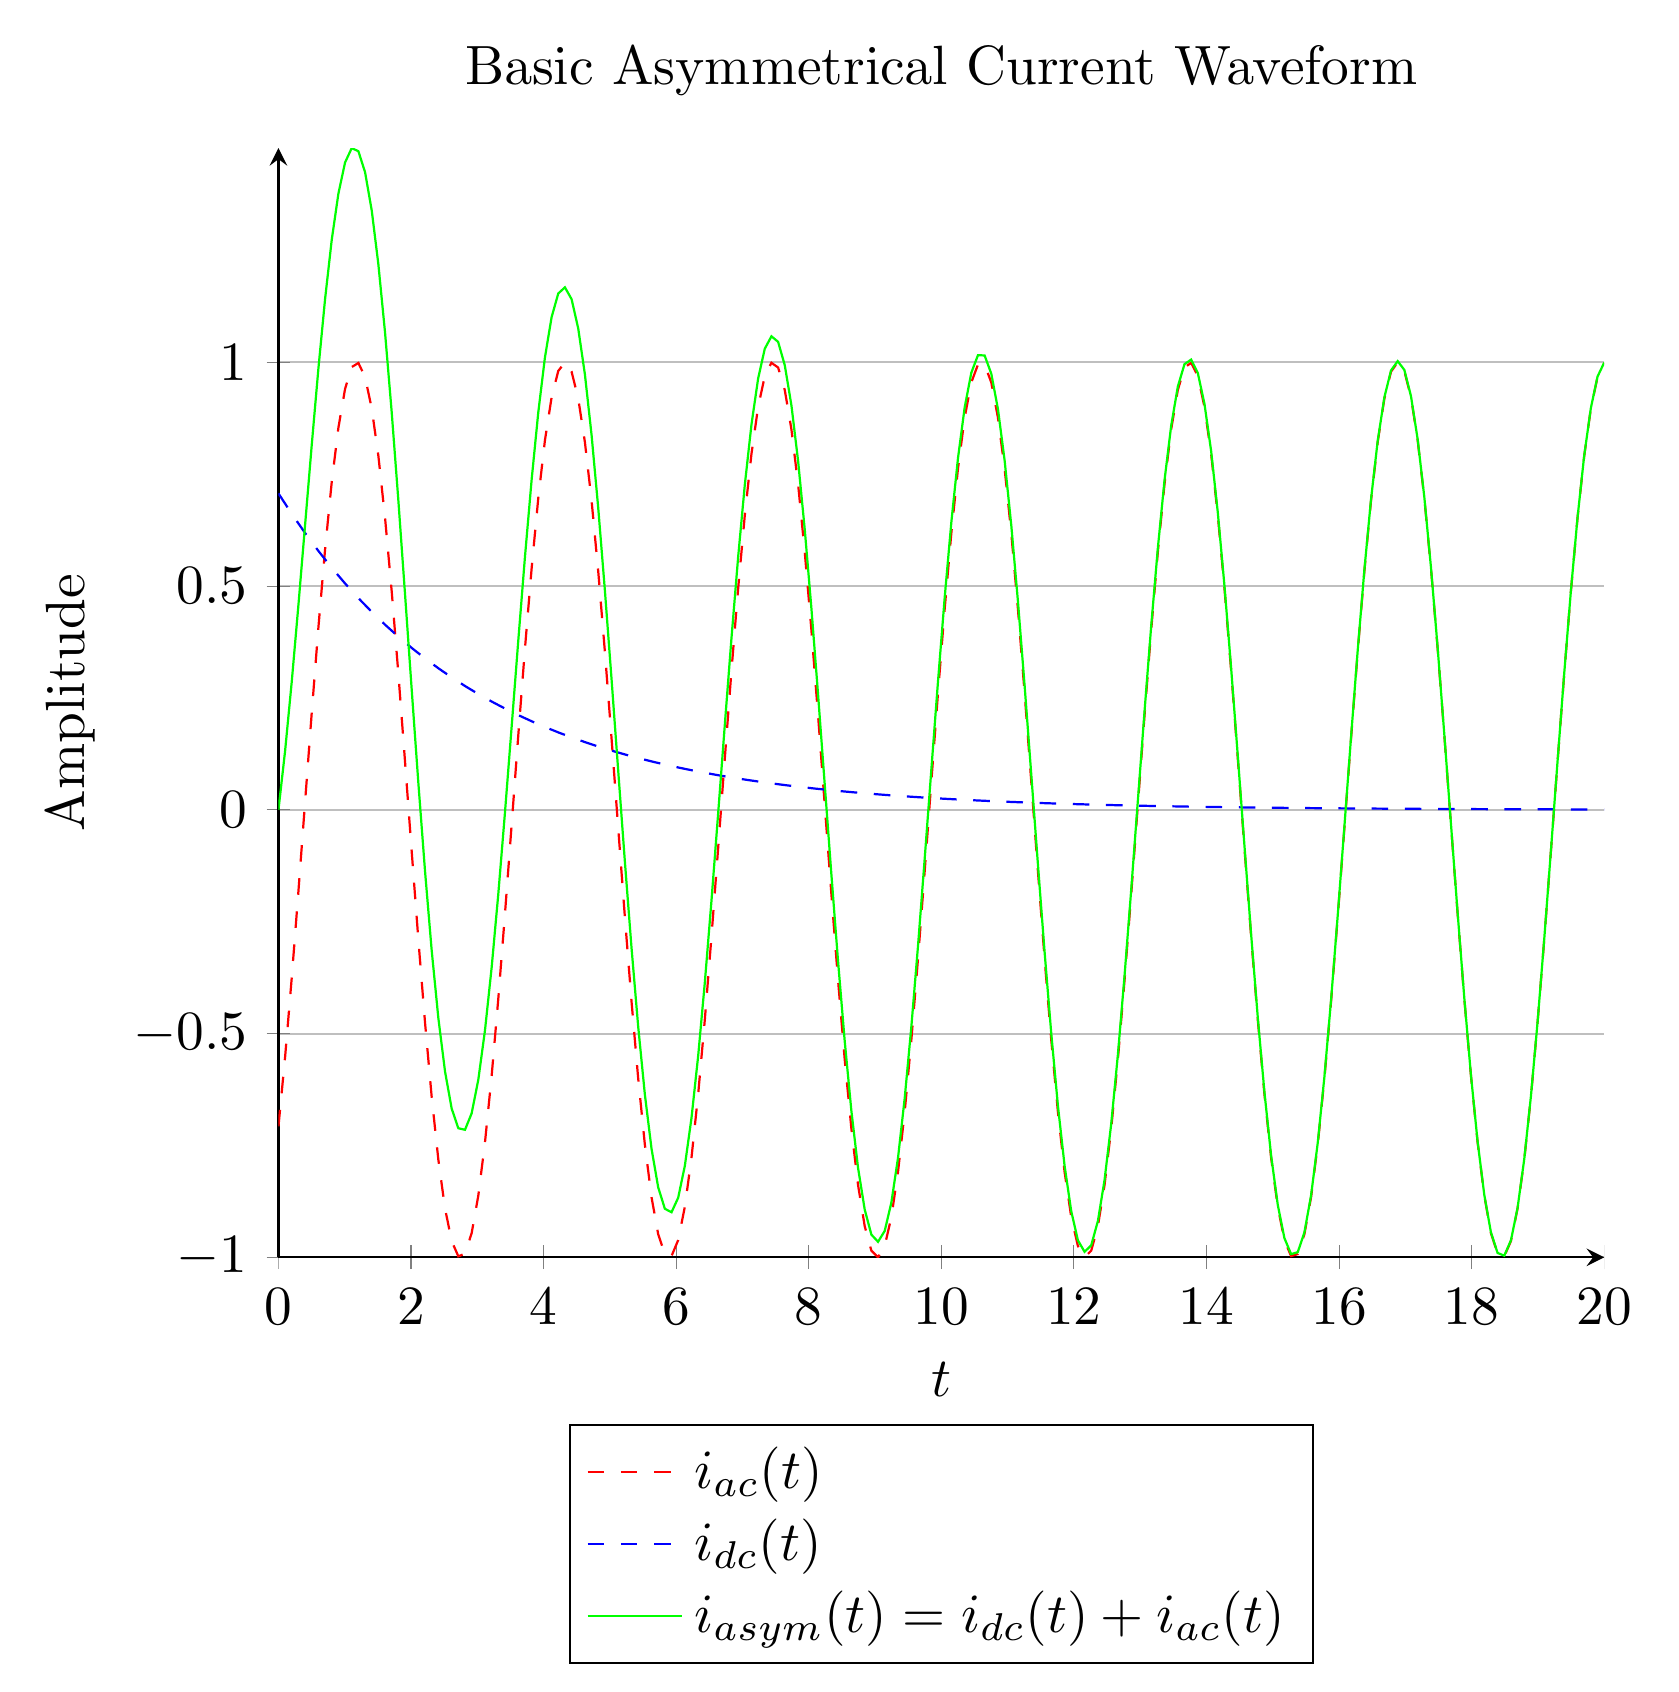
\begin{tikzpicture}[scale = 2]
\begin{axis}[
    title={Basic Asymmetrical Current Waveform},
    xlabel={$t$},
    ylabel={Amplitude},
    axis lines=left,
    ymajorgrids=true,
    legend style={at={(0.5,-0.15)}, anchor=north} ,
    legend cell align=left,
    legend entries={$i_{ac}(t)$, $i_{dc}(t)$, $i_{asym}(t)=i_{dc}(t)+i_{ac}(t)$}
    ]
\addplot[
    red,
    dashed,
    domain=0:20,
    samples=200,
    ] 
	{sin(deg(2*x)-45)};
\addplot[
    blue,
    dashed,
    domain=0:20,
    samples=100,
    ]
    {.707*exp(-(x)/3)};
\addplot[
    green,
    domain=0:20,
    samples=200,
    ]
    {sin(deg(2*x)-45)+.707*exp(-(x)/3)};
\end{axis}
\end{tikzpicture}

\end{document}
